%%%%%%%%%%%%%%%%%%%%%%% file template.tex %%%%%%%%%%%%%%%%%%%%%%%%%
%
% This is a template file for Web of Conferences Journal
%
% Copy it to a new file with a new name and use it as the basis
% for your article
%
%%%%%%%%%%%%%%%%%%%%%%%%%% EDP Science %%%%%%%%%%%%%%%%%%%%%%%%%%%%
%
%%%\documentclass[option]{webofc}
%%% "twocolumn" for typesetting an article in two columns format (default one column)
%
\documentclass{webofc}
\usepackage[varg]{txfonts}   % Web of Conferences font
%
% Put here some packages required or/and some personnal commands
%
%
\usepackage{lineno, blindtext}

\begin{document}
%
\title{A prototype for the evolution of Atlas Eventindex based on Apache Kudu storage}
%
% subtitle is optionnal
%
%%%\subtitle{Do you have a subtitle?\\ If so, write it here}
\begin{linenumbers}
\author{\firstname{Zbigniew} \lastname{Baranowski}\inst{1}\fnsep\thanks{\email{zbigniew.baranowski@cern.ch}} \and
        \firstname{Luca} \lastname{Canali}\inst{1}\fnsep\thanks{\email{luca.canali@cern.ch}} \and
        \firstname{Alvaro} \lastname{Fernandez Casani}\inst{2}\fnsep\thanks{\email{Alvaro.Fernandez@ific.uv.es}} \and
        \firstname{Elizabeth} \lastname{Gallas}\inst{3}\fnsep\thanks{\email{elizabeth.gallas@physics.ox.ac.uk}} \and
        \firstname{Carlos} \lastname{Garcia Montoro}\inst{2}\fnsep\thanks{\email{carlos.garcia@ific.uv.es}} \and
        \firstname{Santiago} \lastname{González de la Hoz}\inst{2}\fnsep\thanks{\email{sgonzale@ific.uv.es}} \and
        \firstname{Julius} \lastname{Hrivnac}\inst{4}\fnsep\thanks{\email{Julius.Hrivnac@cern.ch}} \and
        \firstname{Fedor} \lastname{Prokoshin}\inst{5}\fnsep\thanks{\email{Fedor.Prokoshin@cern.ch}} \and
        \firstname{Grigori} \lastname{Rybkine}\inst{5}\fnsep\thanks{\email{Grigori.Rybkine@cern.ch}} \and
        \firstname{Jose} \lastname{Salt}\inst{5}\fnsep\thanks{\email{Jose.Salt@ific.uv.es}} \and
        \firstname{Javier} \lastname{Sanchez}\inst{5}\fnsep\thanks{\email{Javier.Sanchez@ific.uv.es}} \and
        \firstname{Dario} \lastname{Barberis}\inst{2}\fnsep\thanks{\email{Dario.Barberis@cern.ch}} 
        on behalf of the Atlas Collaboration
        % etc.
}




\institute{CERN, Geneva, Switzerland 
\and
           Insitut de Fisica Corpuscular, Valencia Spain 
\and
           University of Oxford, Oxford, UK
\and
           LAL, Université Paris-Sud and CNRS/IN2P3, Orsay, France
\and
           Universidad Tecnica Federico Santa Maria, Chile 6)Università di Genova and INFN, Genova, Italy
          }

\abstract{%
  The ATLAS EventIndex has been in operation since the beginning of LHC Run 2 in 2015. Like all software projects, its components have been constantly evolving and improving in performance. The main data store in Hadoop, based on MapFiles and HBase, can work for the rest of Run 2 but new solutions are explored for the future. Kudu offers an interesting environment, with a mixture of BigData and relational database features, which look promising at the design level and is used to build a prototype to measure the scaling capabilities as functions of data input rates, total data volumes and data query and retrieval rates. In this paper we report on the selected data schemas and on the current performance measurements with the Kudu prototype.
}
%
\maketitle
%
\section{Introduction}
\label{intro}
The ATLAS EventIndex is a catalogue of all real and simulated events produced by the experiment at all processing stages \cite{RefEI}. 
The system contains hundreds of billions of event records (180 billions of records as of June 2018), each consisting of approximately 1000 bytes. 
The goal of the ATLAS EventIndex is to allow fast and efficient selection of events of interest, based on various criteria, and provide references that point to those events in millions of files scattered in a world-wide distributed computing system.

\section{Motivation for the project evolution}
\label{sec-2}
Current EventIndex was designed in 2012-2013 using best the BigData technology available at that time (Hadoop), implemented in 2014 using MapFiles and HBase, in operation since 2015 with satisfactory results \cite{RefEI2}.
However, the use cases evolved in the meantime and have been extended from event picking and production completeness checks to trigger overlap studies, duplicate event detection and derivation streams (offline triggers) overlaps.
At the same time, the implementation of fast data querying based on traditional relational database involves only a subset of information and is available for real events only \cite{RefORA}
Also, events rate increased steadily throughout Run 2. \newline
BigData technologies advanced, in the meantime and now we have the choice between many different products and options.  
Studies of new data formats and/or new storage technologies \cite{RefZB} concluded that Kudu is the most promising technology for the next few years. Hence this prototype.

\section{Apache Kudu}
\label{sec-3}
Apache Kudu is a next-generation scalable and distributed table-based storage designed for HTAP systems – Hybrid Transactional and Analytical Processing \cite{RefKudu}.
Unlike most of the data formats available for the Hadoop Distributed File System (HDFS)\cite{HADOOP}, Kudu provides indexing and columnar data organization natively – this is to establish a good compromise between random data lookups and analytics performance.
Organization of the data in shared tables with named columns, types and a primary index makes Kudu very attractive for systems with relational data models that need to scale-out.
Apache Kudu is supported by top open-source frameworks for parallel data processing and computation including Apache Spark, Apache Impala, Apache Hive, MapReduce and others.

\section{Concept of the new Atlas EventIndex platform}
\label{sec-4}
\begin{figure}[h]
\centering
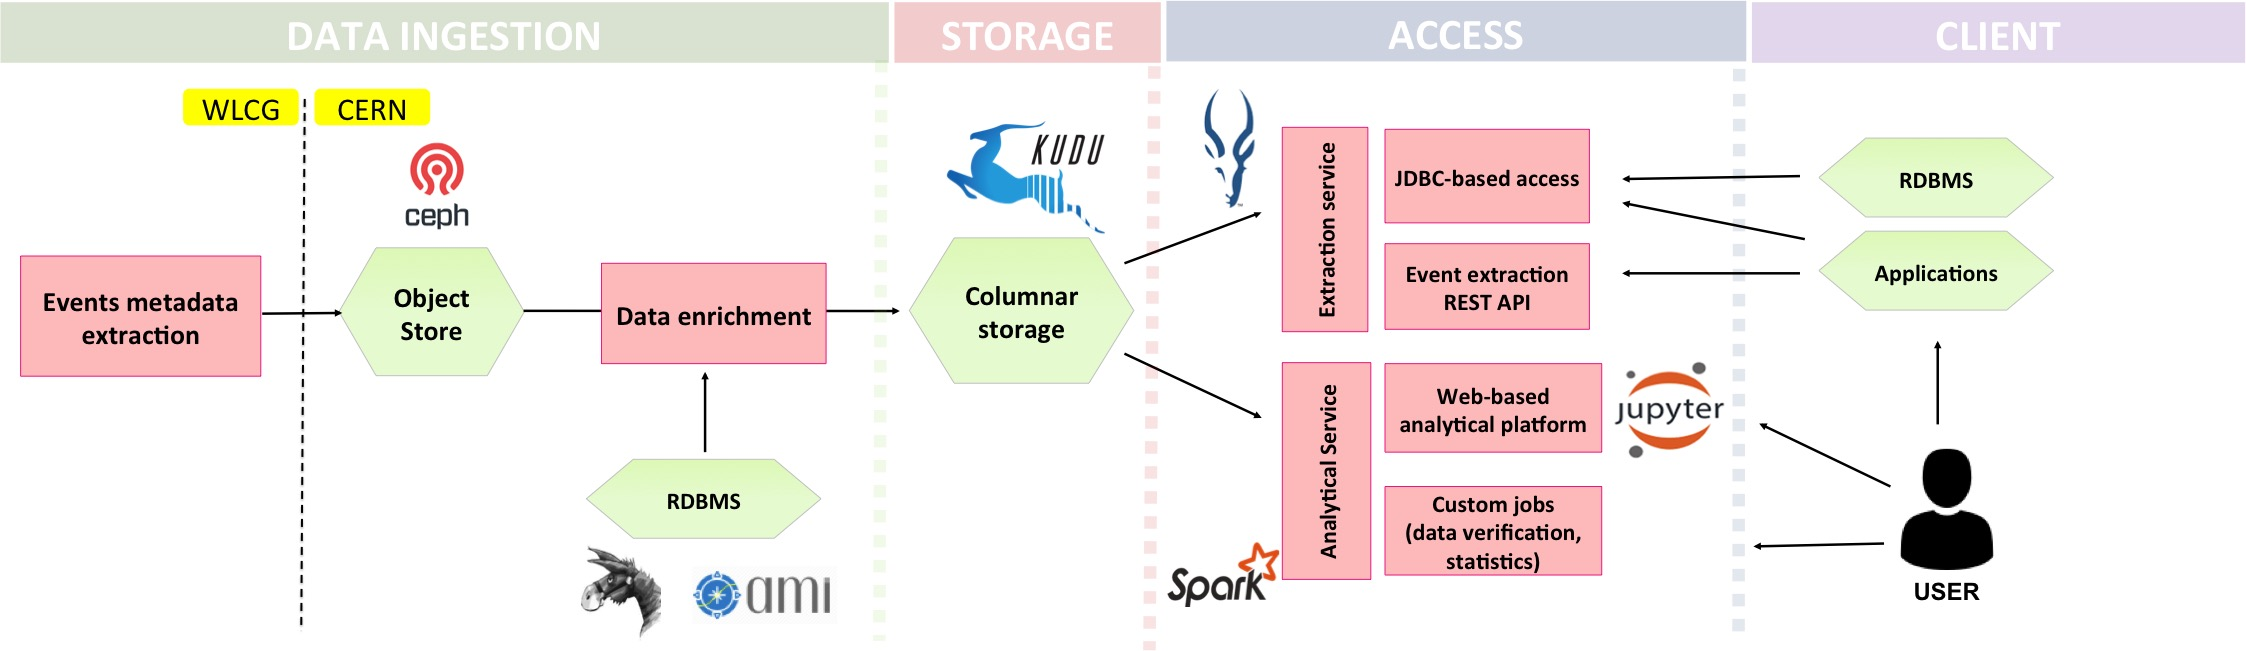
\includegraphics[width=\linewidth,clip]{architecture.jpg}
\caption{The new system architecture}
\label{fig:arch}
\end{figure}
\noindent
Bringing on-board Kudu, a storage supported by many computing frameworks offers to the Atlas EventIndex a possibility to have a modular architecture and increases its flexibility in further evolution. Any module responsible today for one of the functions; data ingestion layer, data access layer or data analytic layer could be replaced with a modern one, without a significant effort. \newline
In the new architecture, we foresee to keep the data ingestion/production part without significant modification. It has been already modernized by introducing a staging area implemented with an object store layer \cite{CEPH} (based on Ceph storage) staging all lately indexed event data from WLCG \cite{WLCG} jobs. The only work foreseen in this area is to build a data pipeline between the object store and the Kudu storage. Such pipeline will need to enrich the data with necessary information regarding trigger state, event provenance etc. from AMI \cite{AMI} and Rucio \cite{Rucio} systems. \newline
\indent
The main modernization touches the data access layer that has to be redesigned in order to fully profit from the functionality and performance offered by Apache Kudu. Notably, the MapReduce framework has to be replaced with low-latency SQL-based frameworks like Apache Impala \cite{Impala}. Impala is well integrated with Kudu and allow to start a lookup events queries within milliseconds. Moreover, the addition of SQL interface on to of Atlas Event Index data will open a possibility to integrate the project with external tools and systems over JDBC protocol. So eventually currently available web front-ends implemented for a relational back-end can be reconnected to the Kudu-based storage. \newline 
As more analytic use cases have been added to the system recently using Apache Spark \cite{Spark}, a modern, highly scale-able and feature-reach data processing engine, would be an obvious chose for implementation of such use cases. With Spark, a lot of complex computations can be expressed imperatively in a high level programming language (Scala, Python or Java) - in a much easier way than the same logic with SQL. Finally, thanks to the available integration of Spark with online Jupyter Notebooks (CERN's SWAN project \cite{SWAN}) we can empower the end-users to write their own analyses and executed on Atlas EventIndex data.
\section{Schema design in Apache Kudu}
\label{sec-5}
When designing a schema in Apache Kudu we had to make decisions on few aspects that ultimately have a great impact on a data access time, scalability and usability of the data stored in Kudu tables. This includes the number of tables and relations between them, choosing appropriate primary keys and partitioning strategies for each of the tables. And finally, data types, encodings and compression algorithms for each of the columns in the tables. \newline
In this section, we will describe the schema for Kudu tables that we prototyped to store the Atlas EventIndex data and criteria that led us to make certain design chooses.
\subsection{Technology constraints}
\label{sec-5-cons}
Along with a certain number of Apache Kudu limitations \cite{KuduLimitations}, there are few that impose certain schema design constraints. Notable, 1) each table has only one index and it is built on a primary key. 2) A table partition is a unit of a table scan parallelism. 3) Each Kudu cluster node can only host 5000 partitions. 4) Partition range has to be known during creation and cannot be modified. 5) The cardinality of key-hash-based sub-partitioning is static and cannot be changed per each partition individually. 6) A table cannot have more than 256 columns. 
\subsection{Partitioning strategy}
\label{sec-5-part}
Knowing the constraints mentioned in the previous sections we had to invoke certain techniques to go around them. \newline
This mainly applies to the non-primary key data access. Such access path requires a scan of all table columns that are part of a query predicate (filtering clause) or projection (selection clause). This quite expensive  (when comparing to the index-based access) process can be executed by multiple parallel processes on the Kudu cluster and effectively reduce greatly the response time. The more partitions (including sub-partitions) the input table has the bigger parallelism can be achieved - this is due to the limitation 2) mentioned in the previous section. For a single range partition, we have decided to have 64 hash-based sub-partitions. This will give at least 64 parallel table scanners when running queries that do not invoke primary key-based access. \newline    
Furthermore, in order to reduce the work done by scanners, the number of rows to be visited by the scanning operation can be narrowed/pruned to those stored in certain partitions. This can happen if a partitioning key is present in a filter predicate of a query. In theory 'runnumber' column from Atlas EventIndex data is the best candidate for a table partition key, as it exists in all the queries and it has very low selectivity, hence only a few partitions will be chosen for scanning. However, since the amount of data per run number is skewed we would have too many almost empty partitions and sub-partitions too. With the respect to the limitation 3) we would quickly reached the maximum number of supported partition. We could group more runs into a single partition in order to keep all partitions with a unified size, however, due to the limitation 4) grouping cannot be done dynamically. To overcome the problem of statically defined partition keys we have to introduce an artificial partition key for event data. Its value is an incremental number, and it has to be controlled by data ingestion supervisor. Once a certain partition is big enough a new one should be created with a key incremented by one. The relation between partition keys and datasets has to be kept in a metadata table and looked up by each query.
\subsection{Tables}
\label{sec-5-tables}
\begin{figure}
\centering
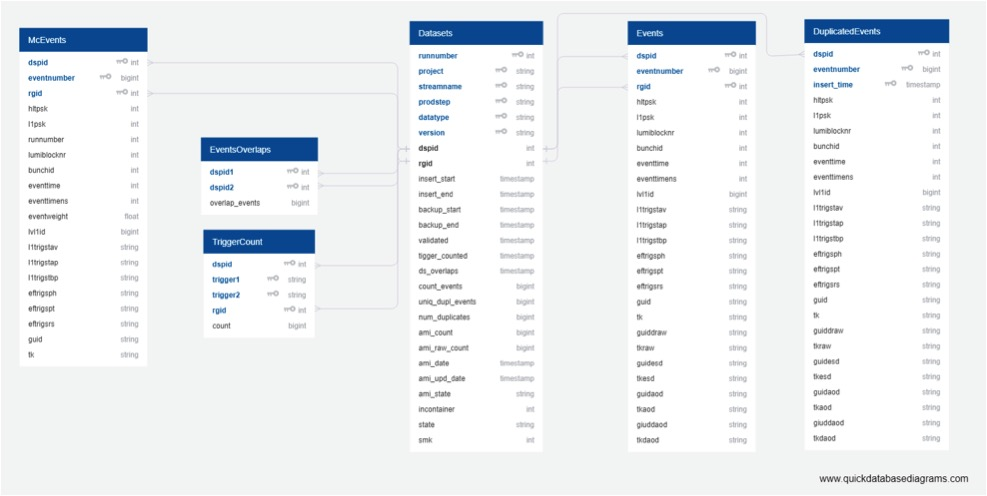
\includegraphics[width=\linewidth,clip]{schema.jpg}
\caption{The prototype schema}
\label{fig:schema}
\end{figure}
Following a process of multiple iterations, we have concluded the following list of tables that should be sufficient to store the system data in an efficient way and provide required functionality: \newline

- \textit{DATASETS} – metadata table, grouping events into datasets. This table assigns a unique id for each dataset, maps each dataset to a partition, provides basic statistics about each dataset, notably the number of events, import time, how much time it took to load it and corresponding statistics copied from AMI system for consistency verification. Full schema of the table can be found in the Table~\ref{tab-1}. Since this table wis expected to not grow significantly in size, it does not have to be partitioned \newline
\begin{table}
\centering
\caption{\textit{Datasets} table schema}
\label{tab-1}
\begin{tabular}{lllll}
\hline
column name & column type & encoding & compression & primary key  \\\hline
runnumber & int & BIT\_SHUFFLE & LZ4 & X \\
project          & string & DICT\_ENCODING  & SNAPPY & X       \\
streamname       & string & DICT\_ENCODING  & SNAPPY & X       \\
prodstep         & string & DICT\_ENCODING  & SNAPPY & X       \\
datatype         & string & DICT\_ENCODING  & SNAPPY & X       \\
version          & string & DICT\_ENCODING  & SNAPPY & X       \\
dspid            & int    & BIT\_SHUFFLE    & LZ4 &            \\
rgid             & int    & BIT\_SHUFFLE    & LZ4 &            \\
insert\_start     & timestamp       & BIT\_SHUFFLE    & LZ4 &   \\
insert\_end       & timestamp       & BIT\_SHUFFLE    & LZ4 &   \\
backup\_start     & timestamp       & BIT\_SHUFFLE    & LZ4 &   \\
backup\_end       & timestamp       & BIT\_SHUFFLE    & LZ4 &   \\
validated        & timestamp       & BIT\_SHUFFLE    & LZ4 &   \\  
count\_events     & bigint          & BIT\_SHUFFLE    & LZ4 &   \\
uniq\_dupl\_events & bigint          & BIT\_SHUFFLE    & LZ4 &   \\
num\_duplicates   & bigint          & BIT\_SHUFFLE    & LZ4 &   \\
tigger\_counted   & int             & BIT\_SHUFFLE    & LZ4 &   \\
ds\_overlaps      & int             & BIT\_SHUFFLE    & LZ4 &   \\
ami\_count        & bigint          & BIT\_SHUFFLE    & LZ4 &   \\
ami\_raw_count    & bigint          & BIT\_SHUFFLE    & LZ4 &   \\
ami\_date         & timestamp       & BIT\_SHUFFLE    & LZ4 &   \\  
ami\_upd_date     & timestamp       & BIT\_SHUFFLE    & LZ4 &   \\
ami\_state        & string          & DICT\_ENCODING  & SNAPPY &\\
inconctainer     & int             & BIT\_SHUFFLE    & LZ4 &   \\  
state            & string          & DICT\_ENCODING  & SNAPPY &\\
smk              & int             & BIT\_SHUFFLE    & LZ4 &   \\\hline
\end{tabular}
\end{table}
\begin{table}
\centering
\caption{\textit{Events} table schema}
\label{tab-2}
\begin{tabular}{lllll}
\hline
column name & column type & encoding & compression & primary key  \\\hline
dspid           & int        & BIT\_SHUFFLE   & LZ4 & X   \\
eventnumber     & bigint     & BIT\_SHUFFLE   & LZ4 & X   \\
rgid            & int        & BIT\_SHUFFLE   & LZ4 & X   \\
hltpsk          & int        & BIT\_SHUFFLE   & LZ4 &     \\
l1psk           & int        & BIT\_SHUFFLE   & LZ4 &     \\
lumiblocknr     & int        & BIT\_SHUFFLE   & LZ4 &     \\
bunchid         & int        & BIT\_SHUFFLE   & LZ4 &     \\
eventtime       & int        & BIT\_SHUFFLE   & LZ4 &     \\
eventtimens     & int        & BIT\_SHUFFLE   & LZ4 &     \\
lvl1id          & bigint     & BIT\_SHUFFLE   & LZ4 &     \\
l1trigmask      & string     & DICT\_ENCODING & SNAPPY &  \\
l1trigchainstav & string     & DICT\_ENCODING & SNAPPY &  \\
l1trigchainstap & string     & DICT\_ENCODING & SNAPPY &  \\
l1trigchainstbp & string     & DICT\_ENCODING & SNAPPY &  \\
eftrigmask      & string     & DICT\_ENCODING & SNAPPY &  \\
eftrigchainsph  & string     & DICT\_ENCODING & SNAPPY &  \\
eftrigchainspt  & string     & DICT\_ENCODING & SNAPPY &  \\
eftrigchainsrs  & string     & DICT\_ENCODING & SNAPPY &  \\
dbraw           & string     & DICT\_ENCODING & SNAPPY &  \\
tkraw           & string     & DICT\_ENCODING & SNAPPY &  \\
dbesd           & string     & DICT\_ENCODING & SNAPPY &  \\
tkesd           & string     & DICT\_ENCODING & SNAPPY &  \\
dbaod           & string     & DICT\_ENCODING & SNAPPY &  \\
tkaod           & string     & DICT\_ENCODING & SNAPPY &  \\
db              & string     & DICT\_ENCODING & SNAPPY &  \\
tk              & string     & DICT\_ENCODING & SNAPPY &  \\
\hline
\end{tabular}
\end{table}


- \textit{EVENTS} – contains metadata about each event. Most of the data access use cases will query this table to obtain information about the events such as: trigger chain, GUID of a file with real event data, a provenance of an event - what files it originated from. The full schema of the table can be found in Table~\ref{tab-2}. Because this table is the subject to grow at a high rate, it has to be partitioned according to rules described in section ~\ref{sec-5-part}. On top of it, we have partitioned it with a hash function into 64 buckets using an event number column, in order to achieve a high degree of parallelism ON evenly distributed data. \newline

- \textit{DUPLICATEDEVENTS} – this table contains all duplicated events that could not be stored in the \textit{events} table due to the primary key violation. It has the exactly the same schema as \textit{events} table except one extra column \textit{insertion\_time} which is a part of the primary key.\newline

- \textit{MCEVENTS} – unlike \textit{events} table, this one stores only simulated events. It has the similar schema as \textit{events}, however some columns related to event provenance information have been dropped since they are not applicable to simulated events. Partitioning strategy should be the same as in case of the \textit{events} table.\newline

- \textit{EVENTSOVERLAP} – the purpose of this table is to store the results of datasets overlap computations - how many events two given datasets are sharing. Therefore it has a basic schema, containing two primary key columns defining datasets id being compared, and a big integer counter column. This table is expected to grow slowly, so no partitioning is needed. \newline

- \textit{TRIGGERCOUNT} – similarly to \textit{eventsoverlap} it should store the results of computations on trigger masks. This table has just 4 columns. Three - \textit{dataset\_id}, \textit{trig1} and \textit{trig2} are making the primary key. The remaining column is just a big integer counter, representing the number of occurrences of the two given triggers within a dataset. Partitioning strategy is the same as in the case of the \textit{events} table, however hashing is dropped, as parallel, non-primary key data access is not required for this table. \newline

\indent
The full schema designed at this stage and used later in performance evaluation is presented in Figure~\ref{fig:schema}.
Notably, we used bit shuffle encoding for numbers and timestamps and dictionary encoding for strings. Regarding the selection of compression algorithm for columns in the tables, we use the following rule: LZ4 for all the columns with bit shuffle encoding and snappy for all the columns with dictionary encoding. All this made a single event record occupying 200 bytes on disk in average (reduced by a factor of 5 in comparison to the original data volume).
\section{Performance of the prototype}
\label{sec-6}
In order to understand the efficiency of the designed schema, a series of performance tests have been concluded with the most important system's use cases: event data ingestion, event look up and analytics on trigger data. 
\subsection{Hardware and software used}
All the performance tests have been concluded on a cluster composed of 12 physical machines, each equipped with 2 CPUs with 8 physical cores with clock speed 2.60GHz, 64 GB of RAM and 48 SAS drives, 4TB each. Apache Kudu was compiled form version 1.7.0 on SLC6 (equivilant to Red Hat 6) Linux distribution. The software was configured to use maximum 10GB of RAM and 10 cores for maintenance tasks. 
\label{sec-6-spec}
\subsection{Data ingestion}
\label{sec-6-di}
\begin{figure}
\centering
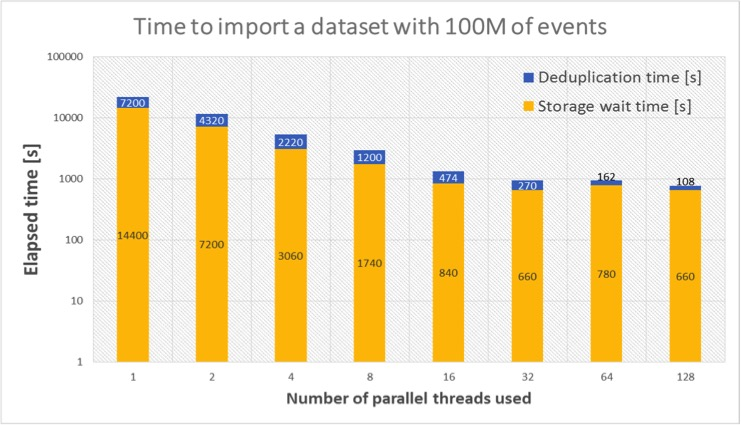
\includegraphics[width=\linewidth,clip]{ingestion.jpg}
\caption{Data ingestion speed measured on representative data set}
\label{fig:ingestion}
\end{figure}
Data loading tests were performed with Apache Spark 2.2.1 using real data from the current production system.
Before loading a dataset to Apache Kudu, duplicated events are filtered out and stored in a dedicated table. The performance tests have been concluded on multiple datasets with random size and a various number of parallel ingestion processes. 
Figure ~\ref{fig:ingestion} shows the results of the set of test performed on a representative dataset with 100M events to demonstrate the scalability of data ingestion 
Measured average writing speed was 5kHz per thread, max overall writing speed to a Kudu cluster was 120kHz. The obtained result is ~10x more than what is needed today by the project.

\subsection{Data access}
\label{sec-6-da}
\begin{figure}
\centering
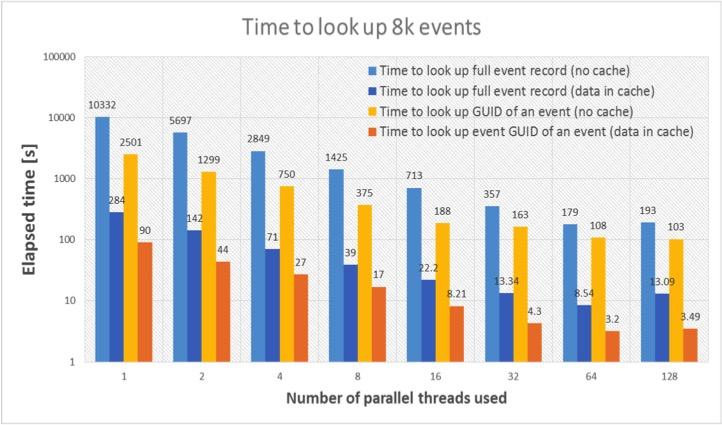
\includegraphics[width=\linewidth,clip]{data_access.jpg}
\caption{Data access representative data set}
\label{fig:access}
\end{figure}
On the Figure~\ref{fig:access} we present the time to look up eight thousands of random events records (full record or just a GUID attribute) from Apache Kudu with a simple client written in Python.
The results for each type of a lookup were grouped into two cases; a pessimistic one (no cache used ) and an optimistic one (all data where lookup from Kudu cache).
The average event lookup time below 1s and ability to handle more then 400 requests per second fully satisfies the future system needs. 

\subsection{Analytics}
\label{sec-6-an}
\begin{figure}
\centering
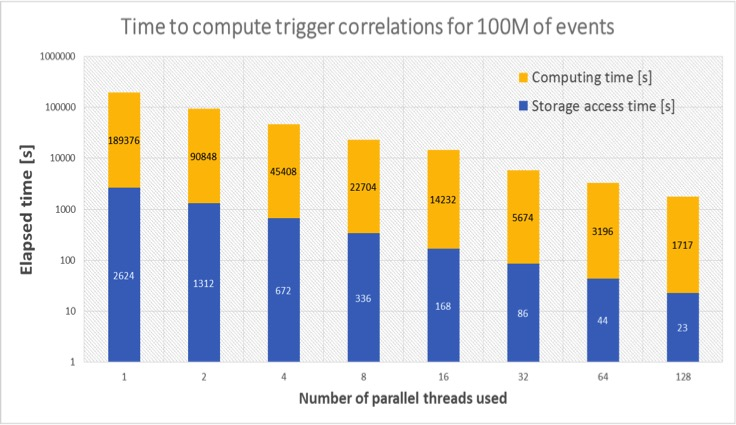
\includegraphics[width=\linewidth,clip]{analytics.jpg}
\caption{Data analytic speed measured on representative data set}
\label{fig:analytics}
\end{figure}
Data analytics tests were performed with Apache Spark 2.2.1 reading Atlas EventIndex from data stored in Apache Kudu.
In Figure~\ref{fig:analytics} are presented execution times for the test case, where we count the occurrences of all combinations of trigger bits pairs within a dataset of 100M events.
The trigger count computation on a Spark cluster takes the majority of the wall time (52 hours), when data retrieval from Kudu is just a small fraction (< 2\%) of it (45 minutes). A single scanner thread could deliver 40k of records per second.


\section{Summary}
\label{sec-7}
The prototype and performed tests have proven that the Atlas EventIndex can profit from migrating the core storage to Apache Kudu in many aspects.
Apache Kudu allows maintaining a hybrid system in a single piece of software. Notably, it enables features like streaming data ingestion, fast data access by index, columnar storage for analytics. 
Eventual migration to a new back-end brings some obvious costs to the project. It requires re-implementation of most of the current components. This, however, should bring a lot of simplification to the code as the vast of the logic needed so far is already built-in in existing frameworks that supports Kudu or in Kudu itself. Scalable data scan performance in combination with modern data processors (Spark, Impala) opens the system to new use cases on a file of data exploration and analytics (like counting trigger correlations).\newline 
\indent
Out of many assets of Apache Kudu, there are also few downsides of it. The biggest one appears to be its maturity and production readiness - the product is available since 2 years, Although we have been running it without any stability problems for months without major problems there are no companies officially using Apache Kudu in production.\newline
\indent
To conclude, feature-wise Apache Kudu appeared to be very strong, fulfiling the Atlas EventIndex project needs for the LHC Run 3. However, from strategic point of view it is an unknown area. Is it there to stay for years? 

\begin{thebibliography}{}

\bibitem{RefEI}
Barberis D et al. 2014 The ATLAS EventIndex: an event catalogue for experiments collecting 
\bibitem{RefEI2}
Barberis D et al. 2015 The ATLAS EventIndex: architecture, design choices, deployment and first operation experience, J. Phys. Conf. Ser. 664 042003
\bibitem{RefORA}
Gallas E et al., 2016, an Oracle-based Event Index for ATLAS, 

\bibitem{RefZB}
Z. Baranowski et al 2017, A study of data representation in Hadoop to optimize data storage and search performance for the ATLAS EventIndex, J. Phys.: Conf. Ser. 898 062020

\bibitem{RefKudu}
Lipcon T et al., 2015, Kudu: Storage for fast analytics on fast data.


\bibitem{HADOOP}
{http://hadoop.apache.org}

\bibitem{CEPH}
Daniel van der Ster, Arne Wiebalck 2014, Building an organic block storage service at CERN
with Ceph ,J. Phys. Conf. Ser. 513 042047


\bibitem{WLCG}
{http://wlcg.web.cern.ch}

\bibitem{AMI}
S Albrand, T Doherty, J Fulachier and F Lambert 2008 The ATLAS Metadata Interface J. Phys.:
Conf. Ser. 119 072003 doi:10.1088/1742-6596/119/7/072003
\bibitem{Rucio}
 V Garonne et al 2014, Rucio – The next generation of large scale
distributed system for ATLAS Data Management, J. Phys.: Conf. Ser. 513 042021
\bibitem{Impala}
{https://impala.apache.org}
\bibitem{Spark}
{https://spark.apache.org}
\bibitem{SWAN}
{https://swan.web.cern.ch}
\bibitem{KuduLimitations}
{https://kudu.apache.org/docs/known\_issues.html}


\end{thebibliography}
\end{linenumbers}
\end{document}

% end of file template.tex

<div id='footer'><table width='100%'><tr><td class='right'><a href='http://fusioninventory.org/'><span class='copyright'>FusionInventory 9.1+1.0 | copyleft <img src='/glpi/plugins/fusioninventory/pics/copyleft.png'/>  2010-2016 by FusionInventory Team</span></a></td></tr></table></div>